% ==================================================
% CHAPTER 4: IMPLEMENTATION AND DELIVERY
% ==================================================

\chapter{Implementation and Delivery}
\label{ch:implementation}

\section{Component Diagrams}

Figure~\ref{fig:components} shows the implemented system as UML components.
The \textbf{Chrome extension} and the \textbf{web app} both require the HTTPS
interface that \textbf{Caddy} provides; Caddy serves the built web app and
requires the REST API that the \textbf{FastAPI backend} provides. The backend
requires Solr's HTTP API, SQL access to two SQLite databases, and three
external interfaces: Cognito for identity, Gemini for summaries and SES for
email. The browser clients also use Cognito directly to sign in.

\begin{figure}[H]
\centering
\begin{tikzpicture}[>={Stealth[length=1.8mm]}]
  \tikzset{comp2/.style={component, text width=#1, minimum height=12mm}, comp2/.default=21mm}
  % ---- components ------------------------------------------------------------
  \node[comp2] (web) at (0, 2.3)  {$\ll$component$\gg$\\\textbf{Web app}\\Svelte SPA};
  \node[comp2] (ext) at (0, 0)  {$\ll$component$\gg$\\\textbf{Extension}\\Chrome MV3};
  \node[comp2=24mm, minimum height=14mm] (eng) at (0,-2.3)
    {$\ll$component$\gg$\\\textbf{Local engine}\\Pyodide $\cdot$ transformers.js\\IndexedDB (encrypted)};
  \node[comp2=17mm, minimum height=30mm] (caddy) at (3.55,0) {$\ll$component$\gg$\\\textbf{Caddy}\\[1mm]TLS, static files, reverse proxy};
  \node[comp2=30mm, minimum height=30mm] (api) at (7.45,0)
    {$\ll$component$\gg$\\\textbf{FastAPI backend}\\[1mm]auth $\cdot$ accounts\\ingest $\cdot$ retrieval\\snippets $\cdot$ summaries\\reports $\cdot$ embeddings\\device keys $\cdot$ backups};
  \node[comp2] (solr) at (11.65, 0.95) {$\ll$component$\gg$\\\textbf{Apache Solr}\\core \texttt{memorylane\_v2}};
  \node[comp2] (sql)  at (11.65,-0.95) {$\ll$component$\gg$\\\textbf{SQLite}\\accounts, reports,\\device keys};
  \node[comp2, dashed] (cog) at (3.55,-3.95) {$\ll$external$\gg$\\\textbf{Amazon Cognito}};
  \node[comp2, dashed] (gem) at (7.45,-3.95) {$\ll$external$\gg$\\\textbf{Google Gemini}};
  \node[comp2, dashed] (ses) at (11.15,-3.95) {$\ll$external$\gg$\\\textbf{Amazon SES}};

  % ---- deployment groupings --------------------------------------------------
  \begin{scope}[on background layer]
    \node[group, dashed, fit=(web)(ext)(eng), inner sep=5pt] (bro) {};
    \node[group, dashed, fit=(caddy)(api)(solr)(sql), inner sep=5pt] (srv) {};
  \end{scope}
  \node[font=\scriptsize\bfseries, anchor=south] at (bro.north) {$\ll$device$\gg$ Browser};
  \node[font=\scriptsize\bfseries, anchor=south] at (srv.north) {$\ll$node$\gg$ AWS EC2 (Docker Compose)};

  % ---- assembly connectors (ball = provided, socket = required) --------------
  % HTTPS: provided by Caddy, required by the web app and the extension
  \coordinate (p1) at (2.15,0);
  \draw (web.east) -- ++(0.25,0) |- ($(p1)+(-0.2,0)$);
  \draw (ext.east) -- ++(0.25,0) |- ($(p1)+(-0.2,0)$);
  \draw (caddy.west |- p1) -- ($(p1)+(0.115,0)$);
  \ballsocket{(p1)}{0}{HTTPS}
  % the website asks the extension for pages kept on the device
  \coordinate (p8) at (0, 1.15);
  \draw (web.south) -- ($(p8)+(0,0.2)$);
  \draw (ext.north) -- ($(p8)+(0,-0.115)$);
  \ballsocket{(p8)}{-90}{site messages}
  % the extension saves and searches through the local engine
  \coordinate (p9) at (0,-1.1);
  \draw (ext.south) -- ($(p9)+(0,0.2)$);
  \draw (eng.north) -- ($(p9)+(0,-0.115)$);
  \ballsocket{(p9)}{-90}{local store}
  % REST API: provided by the backend, required by Caddy
  \coordinate (p2) at (5.15,0);
  \draw (caddy.east |- p2) -- ($(p2)+(-0.2,0)$);
  \draw (api.west |- p2) -- ($(p2)+(0.115,0)$);
  \ballsocket{(p2)}{0}{REST /api}
  % Solr HTTP and SQL: provided by the stores, required by the backend
  \coordinate (p3) at (9.9, 0.95);
  \draw (api.east |- p3) -- ($(p3)+(-0.2,0)$);
  \draw (solr.west) -- ($(p3)+(0.115,0)$);
  \ballsocket{(p3)}{0}{Solr HTTP}
  \coordinate (p4) at (9.9,-0.95);
  \draw (api.east |- p4) -- ($(p4)+(-0.2,0)$);
  \draw (sql.west) -- ($(p4)+(0.115,0)$);
  \ballsocket{(p4)}{0}{SQL}
  % external interfaces required by the backend (socket faces down)
  \coordinate (p5) at (7.45,-2.15);
  \draw (api.south) -- ($(p5)+(0,0.2)$);
  \draw (gem.north) -- ($(p5)+(0,-0.115)$);
  \ballsocket{(p5)}{-90}{Gemini API}
  \coordinate (p6) at (11.15,-2.15);
  \draw ([xshift=10mm]api.south) |- ($(p6)+(0,0.55)$) -- ($(p6)+(0,0.2)$);
  \draw (ses.north) -- ($(p6)+(0,-0.115)$);
  \ballsocket{(p6)}{-90}{SMTP}
  \coordinate (p7) at (3.55,-2.15);
  \draw ([xshift=-10mm]api.south) |- ($(p7)+(0,0.55)$) -- ($(p7)+(0,0.2)$);
  \draw (cog.north) -- ($(p7)+(0,-0.115)$);
  \ballsocket{(p7)}{-90}{OAuth 2.0, JWKS}
  % the browser clients also use Cognito directly (sign-in)
  \draw[->, densely dashed] (bro.south) |- node[font=\tiny, pos=0.75, below] {$\ll$use$\gg$ sign-in} (cog.west);
\end{tikzpicture}

\caption{UML component diagram. A ball is a provided interface, a socket a required one.}
\label{fig:components}
\end{figure}

\section{Deployment Diagrams}

MemoryLane runs on a single AWS EC2 \texttt{c7i-flex.large} instance (2 vCPU,
4\,GB RAM plus 2\,GB swap) in the Mumbai region, with an Elastic IP and the
domain \texttt{memorylane.site}. Figure~\ref{fig:deployment} shows the nodes,
the three Docker containers, their volumes and their connections.

\begin{figure}[H]
\centering
\begin{tikzpicture}[node distance=6mm and 10mm]
  \tikzset{vol/.style={db, minimum width=17mm, minimum height=8mm, font=\scriptsize, fill=white}}
  \node[comp, minimum width=31mm] (caddy) {$\ll$container$\gg$\\\textbf{caddy}\\\scriptsize ports 80, 443\\\scriptsize certificates, web app,\\\scriptsize extension zip, \texttt{/api} proxy};
  \node[comp, right=9mm of caddy, minimum width=29mm] (backend) {$\ll$container$\gg$\\\textbf{backend}\\\scriptsize FastAPI + bge-small\\\scriptsize no published port};
  \node[comp, right=9mm of backend, minimum width=28mm] (solr) {$\ll$container$\gg$\\\textbf{solr} 9.7\\\scriptsize 1\,GB heap\\\scriptsize \texttt{127.0.0.1:8983}};
  \node[vol, below=8mm of caddy] (v1) {caddy\_data};
  \node[vol, below=8mm of backend, xshift=-9.5mm] (v2) {models};
  \node[vol, below=8mm of backend, xshift=9.5mm] (v3) {accounts};
  \node[vol, below=8mm of solr] (v4) {solr\_data};
  \draw[flow] (caddy) -- node[lbl, above] {HTTP} (backend);
  \draw[flow] (backend) -- node[lbl, above] {HTTP} (solr);
  \draw (caddy) -- (v1); \draw (backend) -- (v2); \draw (backend) -- (v3); \draw (solr) -- (v4);
  \begin{scope}[on background layer]
    \node[group, fill=gray!4, fit=(caddy)(solr)(v1)(v4), inner sep=9pt,
          label={[font=\small\bfseries]above:$\ll$node$\gg$ AWS EC2 c7i-flex.large $\cdot$ Docker Compose}] (ec2) {};
  \end{scope}
  \node[box, left=12mm of caddy] (net) {$\ll$device$\gg$\\Browser};
  \draw[flow] (net) -- node[lbl, above] {HTTPS} (caddy);
\end{tikzpicture}
\caption{Deployment diagram: nodes, containers and volumes}
\label{fig:deployment}
\end{figure}

Caddy \cite{caddy} obtains and renews certificates automatically, redirects
HTTP to HTTPS with HSTS, serves the web app and the extension download, sets
the Content Security Policy and proxies \texttt{/api/*} to the backend. Only
ports 80 and 443 are open: the backend is reachable only through Caddy, and
Solr listens on the server's localhost.

\section{Frontend, Backend and Interfaces}

\subsection{Modules}

The repository holds the backend (23 Python modules, about 4{,}000 lines),
the web app (21 Svelte components), the Chrome extension, 566 tests, the
evaluation scripts and the documentation. Table~\ref{tab:modules} lists the
main backend modules.

\begin{table}[H]
\centering
\footnotesize
\begin{tabularx}{\textwidth}{>{\ttfamily}p{0.25\textwidth} L}
\toprule
\textrm{\textbf{Module}} & \textbf{Responsibility} \\
\midrule
main.py & API endpoints, rate limits, log filtering, automatic-save re-check \\
auth.py, accounts.py & Token verification; linking sign-ins by verified email \\
library\_moves.py & Background merge of a library into the linked one \\
ingest.py & The save pipeline, under a per-user write lock \\
cleaning.py, chunking.py & Main-content extraction; overlapping chunks \\
embeddings.py & Model loading, batched passage and cached query embedding \\
retrieval.py & BM25 + KNN, fusion, page grouping, relevance floor \\
query\_intent.py & Site words, time phrases and URLs in queries \\
snippets.py & Sentence snippets for each result \\
solr\_client.py & All Solr access, with the user filter built in \\
page\_filter.py & Rules for pages automatic capture must refuse \\
summarizer.py & On-demand Gemini summaries with a time limit \\
reports.py & Stored problem reports and the email sender \\
youtube\_utils.py & Validated video ids and transcript processing \\
\bottomrule
\end{tabularx}
\caption{Main backend modules}
\label{tab:modules}
\end{table}

\subsection{Browser Extension}

The extension is a Manifest V3 extension \cite{chromemv3} with a popup, an
options page, a background service worker and scripts injected into pages
only when needed. \textbf{Remember this page} injects a content script that
returns the page's HTML, visible text and canonical URL. Single-page
applications such as Reddit keep a stale canonical tag when the address
changes, so a canonical URL is sent only when it describes the current page.
For a YouTube video, the extension fetches the caption track, title, channel,
length and description \emph{inside the user's own tab}, because YouTube
refuses such requests from servers (ADR~0006).

Automatic capture (Figure~\ref{fig:swimlane}) keeps a page only if its address
is not private, the user has read it (30\,s in view, or scrolled halfway after
5\,s), and it reads like content (at least 150 readable words, mostly not
links, no visible password field or large editor, not marked
\texttt{noindex}). The server applies the address rules again, and an
automatic save never rewrites a page already in the library.

\subsection{Backend: Saving}

All saves go through one function, \texttt{ingest\_page}
(Figure~\ref{fig:seq-save}), under the user's write lock. It resolves the
canonical URL and normalises the address (lower-case scheme and host; no
\texttt{www.}, fragment, trailing slash or tracking parameters; sorted
parameters) and derives
\[
\texttt{page\_id} = \mathrm{SHA256}(\texttt{user\_id} \,\|\, \texttt{"|"} \,\|\, \textit{normalised URL})_{[0:32]}.
\]
trafilatura \cite{barbaresi2021trafilatura} extracts the main text, which is
packed into chunks of at most 150 words, each starting with about 30 words of
the previous one. Each chunk is embedded as ``title + chunk'' with
\texttt{BAAI/bge-small-en-v1.5} \cite{xiao2023bge,reimers2019sbert} into a
384-dimensional normalised vector. A content hash and the model name are
stored, so an unchanged page costs one lookup to re-save.

\subsection{Backend: Searching}

BM25 \cite{robertson2009bm25} runs through Solr's edismax parser over
\texttt{title\^{}2 text} with a phrase boost and field syntax disabled, while
the query vector is searched with Solr's HNSW KNN \cite{solr}, using the user
filter as a pre-filter. The two run concurrently. If the query names a site,
time or URL, the rest of the query is searched again within those pages, as a
boost rather than a filter. The ranked lists are fused with Reciprocal Rank
Fusion \cite{cormack2009rrf} (ADR~0002):
\[
\mathrm{RRF}(d) \;=\; \sum_{\ell \,\in\, \text{lists}} \frac{w_\ell}{k + r_\ell(d)},
\qquad k = 60,\; w_\ell = 1 .
\]
Chunks are grouped into pages, each scored by its best chunk
(Section~\ref{sec:bonus}). A page found only by meaning needs a cosine
similarity of at least 0.55 (ADR~0003); a page found by keywords must hold
75\% of the query's words or meet the same bar. Two or three readable
sentences around the best-matching sentence form the snippet.
\textbf{Summarise} asks Google Gemini \cite{gemini} for a summary of one page
with a 20-second limit (ADR~0008). A saved page is untrusted text that may
carry instructions aimed at the model (prompt injection), which no prompt can
rule out, so the design makes a successful injection harmless. The rules are a
fixed system instruction; the request holds only the query and the page, each
in a tag with a random per-request name, and look-alike tags are stripped so
the page cannot close its block and pose as instructions. The model has no
tools and sees nothing but the caller's own page: no user id, address or key.
Its answer is checked before it is shown: links not found in the page are
removed, the length is capped, and an answer that repeats the instruction
(detected by a secret marker) is refused. The web app shows it as plain text.

\subsection{Web Application}

The web app is a Svelte \cite{svelte} single-page application. It signs in
with the authorization-code flow and PKCE (Figure~\ref{fig:seq-signin}), keeps
the access token in memory, and calls the API with a Bearer token, refreshing
once on a \texttt{401}. Deleting is optimistic, with six seconds to undo
(Figure~\ref{fig:state-page}). Voice search uses the browser's speech
recognition. \textbf{Report a problem} shows exactly what will be sent, and the
backend stores the report before emailing it through Amazon SES (ADR~0007).

\subsection{REST API}

\begin{table}[H]
\centering
\footnotesize
\begin{tabularx}{\textwidth}{>{\ttfamily}p{0.11\textwidth} >{\ttfamily}p{0.27\textwidth} L r}
\toprule
\textrm{\textbf{Method}} & \textrm{\textbf{Endpoint}} & \textbf{Purpose} & \textbf{Limit} \\
\midrule
GET & /health & Public status of Solr, model, Gemini & -- \\
POST & /memory & Save or update a page & 60/min \\
GET & /memory/status & Is this URL saved? & 120/min \\
POST & /memory/existing & Which of these pages still exist? & 120/min \\
DELETE & /memory/\{id\} & Delete one page & 60/min \\
GET & /memory/\{id\}/related & Pages closest in meaning & 120/min \\
GET & /memories & Library, newest first & 60/min \\
POST & /search & Hybrid search & 60/min \\
POST & /summarize & Summary of one page & 20/min \\
DELETE & /me/data & Delete all the caller's data & 5/min \\
POST & /reports & Report a problem & 5/hour \\
\bottomrule
\end{tabularx}
\caption{API endpoints. All except \texttt{/health} need a Cognito access token.}
\label{tab:api}
\end{table}

\subsection{Authentication and Data Isolation}

Sign-in is handled by Amazon Cognito \cite{cognito}; MemoryLane never handles
a password. The web app and extension use OAuth 2.0 \cite{rfc6749} with PKCE
\cite{rfc7636} and a public client, so no secret ships to the browser. The
backend verifies each access token's RS256 signature against Cognito's keys,
its expiry, issuer, token type and client id. Google and email sign-ins for
the same \emph{verified} email share one library (ADR~0005), looked up with
the user's own token so the browser cannot fake the email.

Isolation is enforced in the data-access layer: the Solr client adds the
caller's library filter to every query, scan, KNN search and delete, and
refuses to run without a valid id; KNN uses it as a pre-filter; the user id is
part of every page id; a request for another user's page returns \texttt{404},
like a missing page; and no endpoint accepts a user id from the client.
Table~\ref{tab:threats} relates the main threats \cite{owasp2021} to their
mitigations.

\begin{table}[H]
\centering
\footnotesize
\begin{tabularx}{\textwidth}{p{0.29\textwidth} L}
\toprule
\textbf{Threat} & \textbf{Mitigation} \\
\midrule
Reading another user's pages & Library filter in the Solr client; pre-filtered KNN; 404 for foreign ids; isolation tests \\
Forged or replayed tokens & RS256 verification; expiry, issuer, token type and client checks \\
Stolen token via injected script (XSS) & No user HTML rendered; strict CSP; extension tokens out of reach of pages \\
Query injection into Solr & Field syntax disabled; values escaped; ids validated \\
Prompt injection via a saved page & System instruction; randomly tagged data blocks; no tools; output link and leak checks; plain-text display \\
Server-side request forgery & The backend never fetches a client-supplied URL \\
Abuse and resource exhaustion & Per-user rate limits; 5{,}000-page cap; request size limits \\
Sensitive pages captured & Address, reading and content rules; server re-check; one-click removal \\
Personal data in logs & Query strings dropped; Solr and Cognito request URLs not logged \\
Exposed internals & Only ports 80/443 open; Solr bound to localhost \\
\bottomrule
\end{tabularx}
\caption{Threats and mitigations}
\label{tab:threats}
\end{table}

\subsection{Validation and Error Handling}

Inputs are validated at the API boundary with Pydantic models and explicit
limits (URL 2{,}048 characters, text 500\,KB, HTML 3\,MB, query 500
characters). Errors use standard status codes with a JSON \texttt{detail}
message: \texttt{400} missing input, \texttt{401} no valid token,
\texttt{403} page limit, \texttt{404} not found or not yours, \texttt{422}
invalid input or too little text, \texttt{429} rate limit, \texttt{502}/\texttt{503}
an external service failed. The clients turn these into short messages; a
failed delete restores the page, and a refresh that cannot reach Cognito keeps
the session. The complete data flow, from capture to result, is given by
Figures~\ref{fig:dfd1}, \ref{fig:seq-save} and~\ref{fig:seq-search}.

\section{Database and Storage Design}
\label{sec:storage}

\paragraph{Solr.} A saved page is stored as $n$ \emph{chunk documents} in one
core (\texttt{memorylane\_v2}). The key is \texttt{id} =
\texttt{\{page\_id\}::\{chunk\_id\}}, so re-saving overwrites chunks in place
and leftover higher-numbered chunks are deleted. Page-level fields are
repeated on every chunk so that a hit needs no second lookup; chunk~0 also
carries the page vector. Automatic field creation is off, so the schema is
fixed by a setup script.

\begin{table}[H]
\centering
\footnotesize
\begin{tabularx}{\textwidth}{>{\ttfamily}p{0.25\textwidth} p{0.17\textwidth} L}
\toprule
\textrm{\textbf{Field}} & \textbf{Type} & \textbf{Purpose and constraint} \\
\midrule
id & string, key & \texttt{\{page\_id\}::\{chunk\_id\}} \\
user\_id & string, required & Owner's library id; filter on every query \\
page\_id & string & \texttt{sha256(user\_id|normalised URL)[:32]} \\
url, domain & string & Normalised address and host \\
title & text\_en & Page title (weighted $\times 2$ in BM25) \\
text & text\_en & The chunk (stemmed, stop-words removed) \\
description & stored & Meta description or first sentences \\
chunk\_id, total\_chunks & int & Position of the chunk; chunks in the page \\
timestamp & date & When the page was saved \\
content\_hash & string & SHA-256 of the cleaned text \\
embedding\_model & string & Model of the vectors; a change forces re-embedding \\
embedding & vector(384) & Chunk vector, cosine, HNSW index \\
page\_embedding & vector(384) & Mean of the chunk vectors (chunk~0 only) \\
\bottomrule
\end{tabularx}
\caption{Solr schema (\texttt{schema v2})}
\label{tab:schema}
\end{table}

\paragraph{Main queries.} A keyword search is an edismax query with the
filter \texttt{\{!term f=user\_id\}<id>}; a vector search is
\texttt{\{!knn f=embedding topK=50\}} with the same filter as a pre-filter;
the library is a filtered, sorted listing of chunk~0 documents; a delete is a
delete-by-query on \texttt{user\_id} and \texttt{page\_id}.

\paragraph{SQLite.} Two small databases in the \texttt{accounts} volume hold
relational data (Table~\ref{tab:sqlite}). A library is identified by the
\texttt{library} value, which is also the \texttt{user\_id} stored on its Solr
chunks; it is the only link between the two stores. The backend connects to
Solr over HTTP and to SQLite as local files.

\begin{table}[H]
\centering
\footnotesize
\begin{tabularx}{\textwidth}{>{\ttfamily}p{0.2\textwidth} L L}
\toprule
\textrm{\textbf{Table}} & \textbf{Columns (key first)} & \textbf{Relationships and constraints} \\
\midrule
libraries & \underline{email}, library, created\_at & One library per verified email \\
sign\_ins & \underline{sub}, library, email, created\_at, checked\_at & Many sign-ins to one library; re-checked daily \\
library\_moves & \underline{old}, new, created\_at & A library waiting to be merged into another \\
reports & \underline{id}, created\_at, user\_id, email, message, context, sent\_at, attempts, next\_try\_at, last\_error & Indexed by delivery state and by user; deleted with the user's data \\
\bottomrule
\end{tabularx}
\caption{SQLite tables (\texttt{accounts.db}, \texttt{reports.db})}
\label{tab:sqlite}
\end{table}

\section{Screenshots}

\begin{figure}[H]
\centering
\begin{subfigure}[b]{0.52\textwidth}
  \centering
  \screenshot[\textwidth]{figures/extension-popup.png}{extension popup}
  \caption{Popup after a save, with ``Auto-saved today''}
\end{subfigure}\hfill
\begin{subfigure}[b]{0.44\textwidth}
  \centering
  \screenshot[\textwidth]{figures/excluded-sites.png}{excluded sites page}
  \caption{Excluded sites (options page)}
\end{subfigure}
\caption{The Chrome extension}
\label{fig:extension}
\end{figure}

\begin{figure}[H]
\centering
\begin{subfigure}[b]{\textwidth}
  \centering
  \screenshot[0.92\textwidth]{figures/search-results.png}{search results}
  \caption{A search naming a site (``nvidia docs on cuda graphs''): the matching
  snippet with query words highlighted, and the page's summary opened}
\end{subfigure}

\vspace{4mm}
\begin{subfigure}[b]{\textwidth}
  \centering
  \screenshot[0.7\textwidth]{figures/library.png}{library}
  \caption{The library, newest first (a delete button appears on each row on hover)}
\end{subfigure}
\caption{The web application}
\label{fig:webapp}
\end{figure}

\section{Build Configuration and Release}

\begin{table}[H]
\centering
\footnotesize
\begin{tabularx}{\textwidth}{>{\raggedright\arraybackslash}p{0.25\textwidth} L}
\toprule
\textbf{Component} & \textbf{Version} \\
\midrule
Backend runtime & Python 3.11 (\texttt{python:3.11-slim}), CPU-only PyTorch \\
Backend libraries & FastAPI ($\geq$0.104), Sentence Transformers ($\geq$3), trafilatura 2, PyJWT 2, slowapi \\
Search & Apache Solr 9.7 (\texttt{solr:9.7}) \\
Web app & Node 20, Svelte 4.2, Vite 5.3 \\
Web server & Caddy 2 \\
Extension & Manifest V3, version 2.4.2 \\
Models & \texttt{BAAI/bge-small-en-v1.5} (search), Model2Vec \texttt{potion-base-8M} (docs search) \\
\bottomrule
\end{tabularx}
\caption{Versions of the released system}
\label{tab:versions}
\end{table}

\paragraph{Configuration.} Every setting is an environment variable listed
with its default in \texttt{code/src/.env.example}: the Cognito ids, the
Gemini key (optional), SMTP settings (optional), and search settings such as
\texttt{RRF\_K} and \texttt{MIN\_VECTOR\_SIMILARITY}. Secrets live only in the
server's \texttt{.env}, which is never committed.

\paragraph{Build, run and test.} The repository's README gives the commands;
in short:

\begin{lstlisting}[language=bash]
cd code/src && cp .env.example .env          # fill in the Cognito ids
docker compose up -d solr
docker compose exec solr solr create -c memorylane_v2 -d _default
CORE_NAME=memorylane_v2 ./scripts/setup_solr.sh
docker compose up -d --build                  # backend + caddy (builds the web app)
python -m pytest -q                           # backend tests
cd frontend && npm test && npm run check      # frontend tests and type check
\end{lstlisting}

\paragraph{Sample data.} The SciFact corpus in
\texttt{code/src/evaluation/scifact\_data} can be indexed into a separate core
with \texttt{python -m evaluation.scifact\_ingest}, and
\texttt{python -m evaluation.scifact\_evaluate} writes every metric with its
confidence interval to \texttt{scifact\_report.json}.

\paragraph{Release workflow and CI.} GitHub Actions runs the backend and
frontend test suites on every push and pull request
(\texttt{.github/workflows/ci.yml}) and builds the documentation in strict
mode when it changes. A release is a push to \texttt{master} followed, on the
server, by \texttt{git pull} and \texttt{docker compose up -d --build}; the
Caddy image builds the web app and zips the extension during that build, so
what is served always matches the deployed code. Schema changes are applied by
script before the code that needs them. Backups are EBS snapshots.

\section{User Documentation and Access}

\begin{table}[H]
\centering
\footnotesize
\begin{tabularx}{\textwidth}{p{0.24\textwidth} L}
\toprule
\textbf{Resource} & \textbf{Location} \\
\midrule
Live application & \url{https://memorylane.site} \\
Extension download and installation & \url{https://memorylane.site/extension} \\
Documentation & \url{https://rabeeh18.github.io/ucs503p-202627-MemoryLane/} \\
Source code & \url{https://github.com/rabeeh18/ucs503p-202627-MemoryLane} \\
\bottomrule
\end{tabularx}
\caption{Access to the delivered system}
\label{tab:resources}
\end{table}

The documentation site \cite{mkdocsmaterial} has a step-by-step
\textbf{Tutorial}, a \textbf{Usage Guide} for every feature, installation and
configuration guides, the API reference, architecture and decision records,
the evaluation and a glossary. Its search box finds sections by meaning as
well as keywords, using Model2Vec \cite{model2vec} static embeddings computed
at build time. The repository's \texttt{README.md}, \texttt{MANIFEST.md} and
\texttt{LICENSE} (MIT) describe the project, its files and its terms. This
report describes the version on the \texttt{master} branch on 26~November
2026, with extension version 2.4.2.

\section{Iterations and Changes}
\label{sec:iterations}

MemoryLane was built iteratively \cite{sommerville2016se}, and each update
was posted on the course forum and discussed with the supervisor
(Figure~\ref{fig:timeline}). Supervisor feedback shaped several decisions: the
question of storing full text versus snapshots (full text was kept, for better
summaries) and the move to Apache Solr discussed at the 24~August lab. The
next steps we set in those discussions, a dynamic number of results and a
lower LLM cost, later became the relevance floor and on-demand summaries.

\begin{figure}[H]
\centering
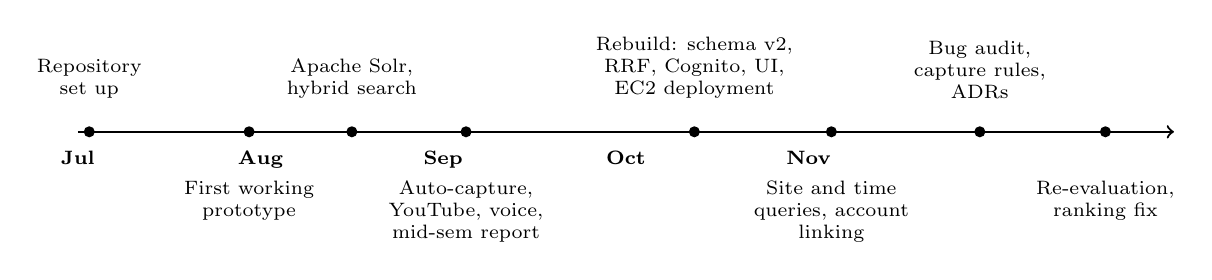
\begin{tikzpicture}[x=1.45cm]
  \draw[thick,->] (0,0) -- (9.6,0);
  \foreach \x/\m in {0/Jul, 1.6/Aug, 3.2/Sep, 4.8/Oct, 6.4/Nov}
    \node[font=\scriptsize\bfseries, below] at (\x,-0.12) {\m};
  \foreach \x in {0.1,1.5,2.4,3.4,5.4,6.6,7.9,9.0}
    \fill (\x,0) circle (2pt);
  \node[font=\scriptsize, align=center, above=3mm] at (0.1,0) {Repository\\ set up};
  \node[font=\scriptsize, align=center, below=5mm] at (1.5,0) {First working\\ prototype};
  \node[font=\scriptsize, align=center, above=3mm] at (2.4,0) {Apache Solr,\\ hybrid search};
  \node[font=\scriptsize, align=center, below=5mm] at (3.4,0) {Auto-capture,\\ YouTube, voice,\\ mid-sem report};
  \node[font=\scriptsize, align=center, above=3mm] at (5.4,0) {Rebuild: schema v2,\\ RRF, Cognito, UI,\\ EC2 deployment};
  \node[font=\scriptsize, align=center, below=5mm] at (6.6,0) {Site and time\\ queries, account\\ linking};
  \node[font=\scriptsize, align=center, above=3mm] at (7.9,0) {Bug audit,\\ capture rules,\\ ADRs};
  \node[font=\scriptsize, align=center, below=5mm] at (9.0,0) {Re-evaluation,\\ ranking fix};
\end{tikzpicture}
\caption{Project timeline, July--November 2026}
\label{fig:timeline}
\end{figure}

\begin{table}[H]
\centering
\footnotesize
\begin{tabularx}{\textwidth}{>{\raggedright\arraybackslash}p{0.2\textwidth} L L}
\toprule
\textbf{Aspect} & \textbf{Prototype (mid-semester)} & \textbf{Final product} \\
\midrule
Users & One user, no sign-in & Multi-user, Amazon Cognito, linked by verified email \\
Capture & TamperMonkey script, then a basic extension & Manifest V3 extension with automatic-capture rules \\
Deployment & Local Docker & AWS EC2, Docker Compose, Caddy with HTTPS \\
Embedding model & \texttt{all-MiniLM-L6-v2} & \texttt{bge-small-en-v1.5} with a query instruction \\
Chunking & 300--500 words & 150 words, 30-word overlap, title embedded \\
Fusion & Min-max scores, 0.5\,/\,0.5 & Reciprocal Rank Fusion ($k=60$) \\
Query understanding & None & Site words, time phrases and URLs \\
Result quality & Best chunk per page, fixed result count & Relevance floor, keyword coverage, sentence snippets \\
YouTube & Server-side transcripts & Captions fetched in the user's browser \\
Library & None & Library page, delete with undo, delete all data \\
Tests & A few scripts & 566 automated tests in CI \\
Documentation & README & 48-page site, 11 decision records, meaning-based search \\
Evaluation & 3 metrics, 3 runs & 7 quality metrics, latency, bootstrap intervals, 5 runs \\
\bottomrule
\end{tabularx}
\caption{The prototype and the final product}
\label{tab:prototype-vs-final}
\end{table}

\paragraph{Completed, partial and omitted features.} All twelve functional
requirements are delivered. Two built features were \emph{omitted} on
purpose: the library map (a clustered view of the library) and ``Export my
data'' were removed as costly or little used (ADRs 0009, 0010). The optional
cross-encoder reranker is implemented but left off on the live server to save
memory, so it is \emph{partial}. Importing existing history or bookmarks was
considered and not started.
